\section{Graphics programming}
Typically deals with how to define 3D scene, with virtual camera and how to create a 2D projection of the 3D scene

\subsection*{Real time vs offline rendering}
\textbf{Real time} used in games, scene must be updated 30-60 fps here is speed > image quality, but today hardware can do pretty much both. \textbf{offline} rendering is used for animated movies and visual effects and is not meant to be used interactively. In this field rendering of a single frame can take several hours. Image quality > speed in this case. Movie production uses clusters to calculate the renders in parallel.

\subsection*{How do we draw}
Version 1, traditionally used mainly in offline rendering

\begin{example}{Version 1}
\begin{lstlisting}[language=]
For every pixel on screen
	Query all objects to be drawn,
	to determine the correct color for that pixel "Ray tracing"
end
\end{lstlisting}
\end{example}

Version 2, most common method for real time rendering
\begin{example}{Version 2}
\begin{lstlisting}[language=]
For every object
	Draw the object to the screen,
	by setting the correct colors for the affected pixels
end
\end{lstlisting}
\end{example}


\subsection*{Representation}
\textbf{Polygonal meshes} are typically used for representing 3D models, using collections of vertices, edges and faces. Faces can be arbitrary polygons but we typically split them in triangles so the implementation gets simpler. 

\subsection*{Vertex data}
Each vertex in the polygonal mesh has one or several attributes such as:

\begin{itemize}
	\item Position
	\item Color
	\item Normal vector
	\item texture coordinate
\end{itemize}

The vertex data is typically loaded on the CPU and uploaded memory that is accessible from the GPU via \textbf{buffer objects}.

\subsection*{Transforms}
Transforms are used to manipulate positions orientation, size and shape of object in the 2D/3D scene. Transforms are also used to define a virtual camera and go from one coordinate system to another. Theses transformations are often represented as 3 by 3 or 4 by 4 matrices. Examples of some basic transforms:

\begin{itemize}
	\item Translation
	\item Rotation
	\item Scaling
\end{itemize}

\subsection*{Coordinate systems}
The OpenGL pipeline has 6 different coordinate systems

\begin{itemize}
	\item Object 
	\item World
	\item Eye (or camera)
	\item Clip
	\item Normalized devices
	\item Window (or screen)
\end{itemize}

\subsection*{Surface normal}
A normal vector is a perpendicular vector to the surface that points outwards from the surface. It describes a local orientation of a surface at some vertex or face. Super important to lighting. Useful to know if the surface is pointing towards me or not 

Can visualize it with RGB vector for example.

\subsection*{Shaders}
In real time rendering is shader a small program that is compiled on the CPU and executed on the GPU. Common use is to apply transformations on vertices and compute and compute the level of light and colors of the fragments/pixel candidates. Using different shader or shader input can drastically change the visual appearance of a 3D object. 

\subsection*{The programmable graphics pipeline}

\textcolor{red}{create illustrator image} 

\subsection*{OpenGL}
OpenGL is a cross-platform low level API for rendering of 2D and 3D graphics. It is 
state-based and maintain a currents state of things (what shader is being used etc). The first version was launched in 1992. Used in many applications such as: games, simulations, scientific visualizations, CAD, mobile applications, VR etc.  
OpenGL only handles rendering and not any input or windowing. It is callable form many programming languages such as: C, C++, Python, Java, C\#, JS, Rust and more. It comes in many variations: 
\begin{itemize}
	\item OpenGL for desktop
	\item OpenGL ES for embedded systems
	\item WebGl for web browsing 3D graphics.
\end{itemize}
Alternatives to OpenGL are: Metal (MacOS), Vulkan and DirectX (Microsoft).

OpenGL functions are executed in the host CPU application and responsible for: 

\begin{itemize}
	\item Creating and initializing buffers, shaders, textures etc.
	\item Upload data to GPU accessible memory. 
	\item Configure the render state.
	\item Submit drew calls.
	\item Clear and swapping buffers.
\end{itemize}


\subsection*{The CPU and GPU}
We here present a couple of very simplified "algorithms" for drawing a object:

\begin{example}{"Immediate mode" rendering} 
\begin{lstlisting}[language=]
initialize_system();
for (each object to be drawn){
	
	o = generate_object();
	draw_object(o);
}
cleanup();
\end{lstlisting}
\end{example}	

\begin{example}{"Retained mode" rendering} 
\begin{lstlisting}[language=]
initialize_system();
for (each object to be drawn){
	
	o = generate_object();
	store_object(o);
}

draw_all_objects();
cleanup();
\end{lstlisting}
\end{example}	

\begin{example}{"Retained mode" rendering} 
\begin{lstlisting}[language=]
initialize_system();
for (each object to be drawn){
	
	o = generate_object();
	store_object(o);
}
send_object_to_GPU(); 
//Can be a bottleneck, if we want to draw the same object multiple times
// it is beneficial to only send them once to the GPU

draw_all_objects();
cleanup();
\end{lstlisting}
\end{example}	

\subsection*{Utility libraries}
Since OpenGL is only used for rendering, we need to use a variety of so called utility libraries in our applications. Here are the ones we will be using in the labs:

\begin{itemize}
	\item GLFW create and manage window.
	\item GLEW extension loader.
	\item GLM mathematics library.
	\item ImGui GUI.
\end{itemize}


\textbf{GLFW} gives us an interface between the windowing system and graphics system and allows us to create a window, executes the rendering loop and setup a mouse and keyboard interaction. \textbf{GLEW} is a cross-platform C/C++ library loading OpenGL extensions. GLEW will search for and pull in all the OpenGL extensions that we need/supported, \textbf{GLM} is mathematics library for graphical programming and provides vector and matrix datatypes, transforms, quaternions, noise functions and much, much more. It is used in the host/CPU for C++ applications only. \textbf{ImGui} is a GUI library that is useful for tweaking rendering parameters. 


\subsection*{Vertex buffer objects (VBOs)}
VBO's are used for uploading arrays of vertex data/attributes to the GPU memory. Before we submit a draw call we must bind the VBOs. We can split our VBOs into groups of each vertex attribute or interleave several vertex attributes in one single VBO (this us usually more efficient).

\subsection*{Vertex array objects (VAOs)}
A VAO stores references to one or several VBOs along with their states and configurations. At drawing we only have to bind the VAO, it simplifies the code so we don't have to bind and configure the VBOs separately at each draw call. Recent OpenGL core profiles require the use of VAOs


\subsection*{glDraqArrays and glDrawElements}
These are draw commands for rendering graphics primitives: lines, points and triangles from array data stored in VBOs or VAOs. 

\begin{example}{Example: }
\begin{lstlisting}[language=]
void drawTriangle(GLuint program, GLuint vao)
{
  glUseProgram(program);
 
  glBindVertexArray(vao);
  glDrawArrays(GL_TRIANGLES, 0, 3);
  glBindVertexArray(0);
  glUseProgram(0);
}
\end{lstlisting}

\end{example}	


\subsection*{OpenGL primitives}
The following primitives are the basic building blocks in OpenGL applications: 
\begin{itemize}
	\item Point sprites: GL\_POINTS
	\item Lines: GL\_LINES, GL\_LINE\_STRIP, GL\_LINE\_LOOP
	\item Triangles: GL\_TRIANGLE, GL\_TRIANGLE\_STRIP, GL\_TRIANGLE\_FAN
\end{itemize}

\begin{figure}[ht!]
\centering
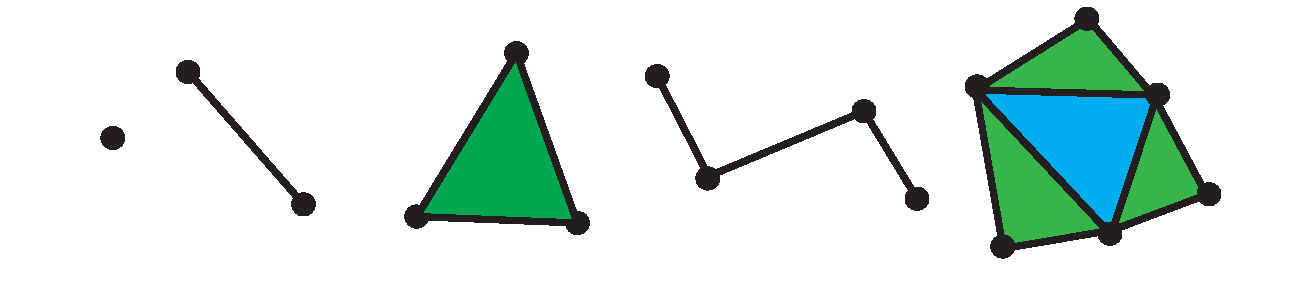
\includegraphics[width=100mm]{figures/primitives.pdf}
\caption{Example of caption}
\label{fig:example}
\end{figure}

\subsection*{GLSL OpenGL shading language}
GLSL is a high-level, cross-platform shading language for real-time rendering. It is based on the C-programming language and uses similar naming conventions, data-types and control structures. Following data-types and functions are built in:
\begin{itemize}
	\item vector and matrix types
	\item various math and utility functions for graphics programming, dot, cross, max, normalize etc.
	\item texture lookup functions
\end{itemize}

\subsection*{Shader types}
OpenGL support six different types of shaders. Vertex and fragment shaders are covered in this course.
\begin{itemize}
	\item \textbf{Vertex}
	\item \textbf{Fragment}
	\item Geometry
	\item Tesselation control
	\item Tesselation evaluation
	\item Compute
\end{itemize}

\subsection*{The vertex and fragment shader }
An example of the task the vertex shader have is to apply color and transformation on the input vertices and pass varying data the the fragment shader. 

The fragment shader takes \textbf{uniforms} and interpolated data from the vertex shader and rasterize as input. It then computes the final color of fragments called pixel candidates by evaluating lightning equations. 

The GLSL source code is typically stored in plain ASCII text files with the suffixes *.vert for vertex shaders and *.frag for fragment shaders. When the program starts the host application loads the GLSL source files into strings and then compile them into shaders that can be executed on the GPU.

\subsection*{Workflow - Creating, compiling and linking}
The main steps in Creating, compiling and linking GLSL shaders are listed here:

\begin{enumerate}
	\item Read vertex and framgent shaders source files into strings
	\item Create vertex shader object from the vertex shader source string
	\item Create fragment shader object from the fragment shader string
	\item Compile the program
	\item Link the compiled program and check for errors
	\item De-attach and delete the shader object
\end{enumerate}


\begin{example}{Example: GLSL vertex shader}
\begin{lstlisting}[language=]
#version 330 // specifies the GLSL version
in vec4 a_position; // input vertex position
void main() {
  // just sets the output vertex position 
  // to the input vertex position 
  gl_Position = a_position;
}
50
GLSL fragment shader 
(triangle.frag)
#version 330
out vec4 frag_color; // output fragment color
void main() {
  // sets the output fragment color to white
  frag_color = vec4(1.0, 1.0, 1.0, 1.0);
}
\end{lstlisting}
\end{example}	

The variables types that are used for communicating with shaders are of three types:

\begin{itemize}
	\item Attribute
	\item Varying
	\item Uniform
\end{itemize}

\textbf{Attribute} variables can be accessed via the \textcolor{blue}{\textbf{in}} qualifier. \textbf{Varying variables} provides an interface for passing colors, normals, texture coordinates and other data between the vertex shader and the fragment shader. Varying data is be default linearly interpolated over the geometric primitive. The vertex shader uses the \textcolor{blue}{\textbf{out}} qualifier to pass varying data the fragment shader. The fragment shader accesses the data via the \textcolor{blue}{\textbf{in}} qualifier and writes an output via the \textcolor{blue}{\textbf{out}} qualifier. \textbf{Uniform variables} are used for data that should be constant for all vertices and fragments. Examples of such data are: transforms, material properties (color, opacity, etc), light sources, texture samplers, time and flags for enabling/disabling parts of the shading. \textbf{Uniform} variables can be accessed in both the vertex and fragment shader via the \textcolor{blue}{\textbf{uniform}} qualifier. 

\subsection*{Transforms in shader based OpenGL}
Typically is the transform constructed in the host C++ program using GLM and passed to the vertex shader as uniform variables. On the GPU side, the vertex shader applies the transforms on the incoming vertex data. 


